\subsection{Red neuronal artificial}
Una red neuronal (RN) es un modelo constituido por un
n\'umero masivo de unidades de c\'omputo de dise\~no simple
conocidas como neuronas. La figura \ref{fig:neurona}  muestra un ejemplo
de una neurona.

\begin{figure}[H]
	\centering
	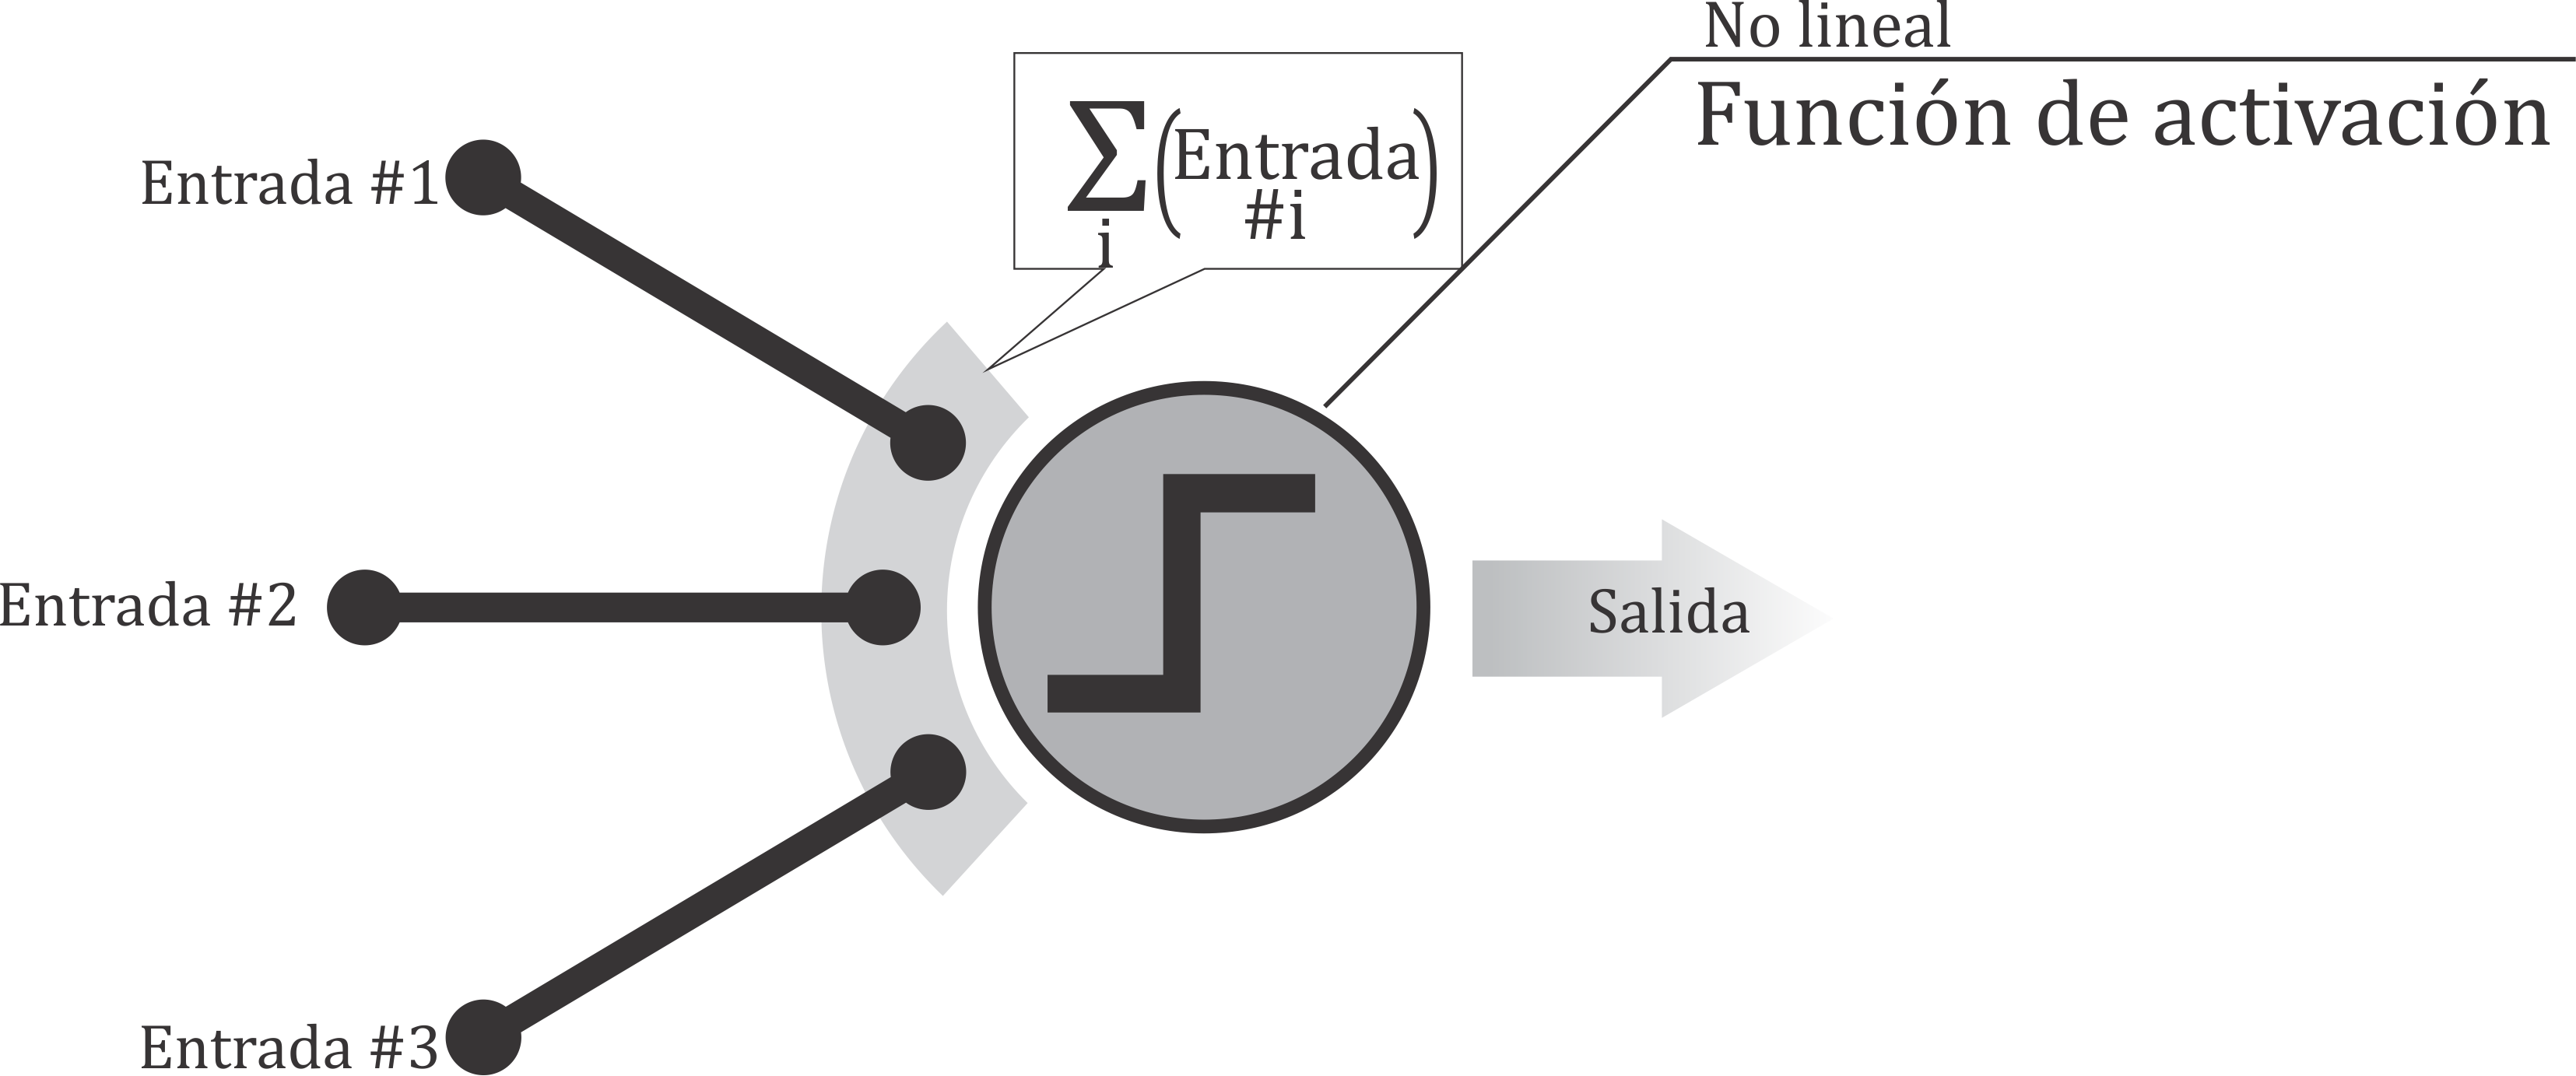
\includegraphics[width=5cm]{img/fig_neuron.png}
	\caption{Modelo de unidad de c\'omputo simple, neurona.}
	\label{fig:neurona}
\end{figure}

Todas las se\~nales que ingresan a la neurona son sumadas,
al final la amplitud de la se\~nal de salida de la neurona se
determina por una funci\'on de activaci\'on no-lineal $\sigma(z)$. Aqu\'i
se hace uso de la siguiente ecuaci\'on: 

\begin{equation}
	\sigma(z)=\frac{1-e^{-kz}}{1+e^{-kz}}
\end{equation}

La figura \ref{fig:activa} considera $k=1$, conforme $k\rightarrow\infty$ la funci\'on
$\sigma(z)$ se comporta como una funci\'on escal\'on. Es conveniente
considerar a la funci\'on de activaci\'on con una inclinaci\'on
moderada con esto la respuesta de la red estar\'a dentro de un
rango de valores $\left[1-,1\right]\subset\Re$, lo anterior muestra la diferenciabilidad
de la red.

\begin{figure}[H]
	\centering
	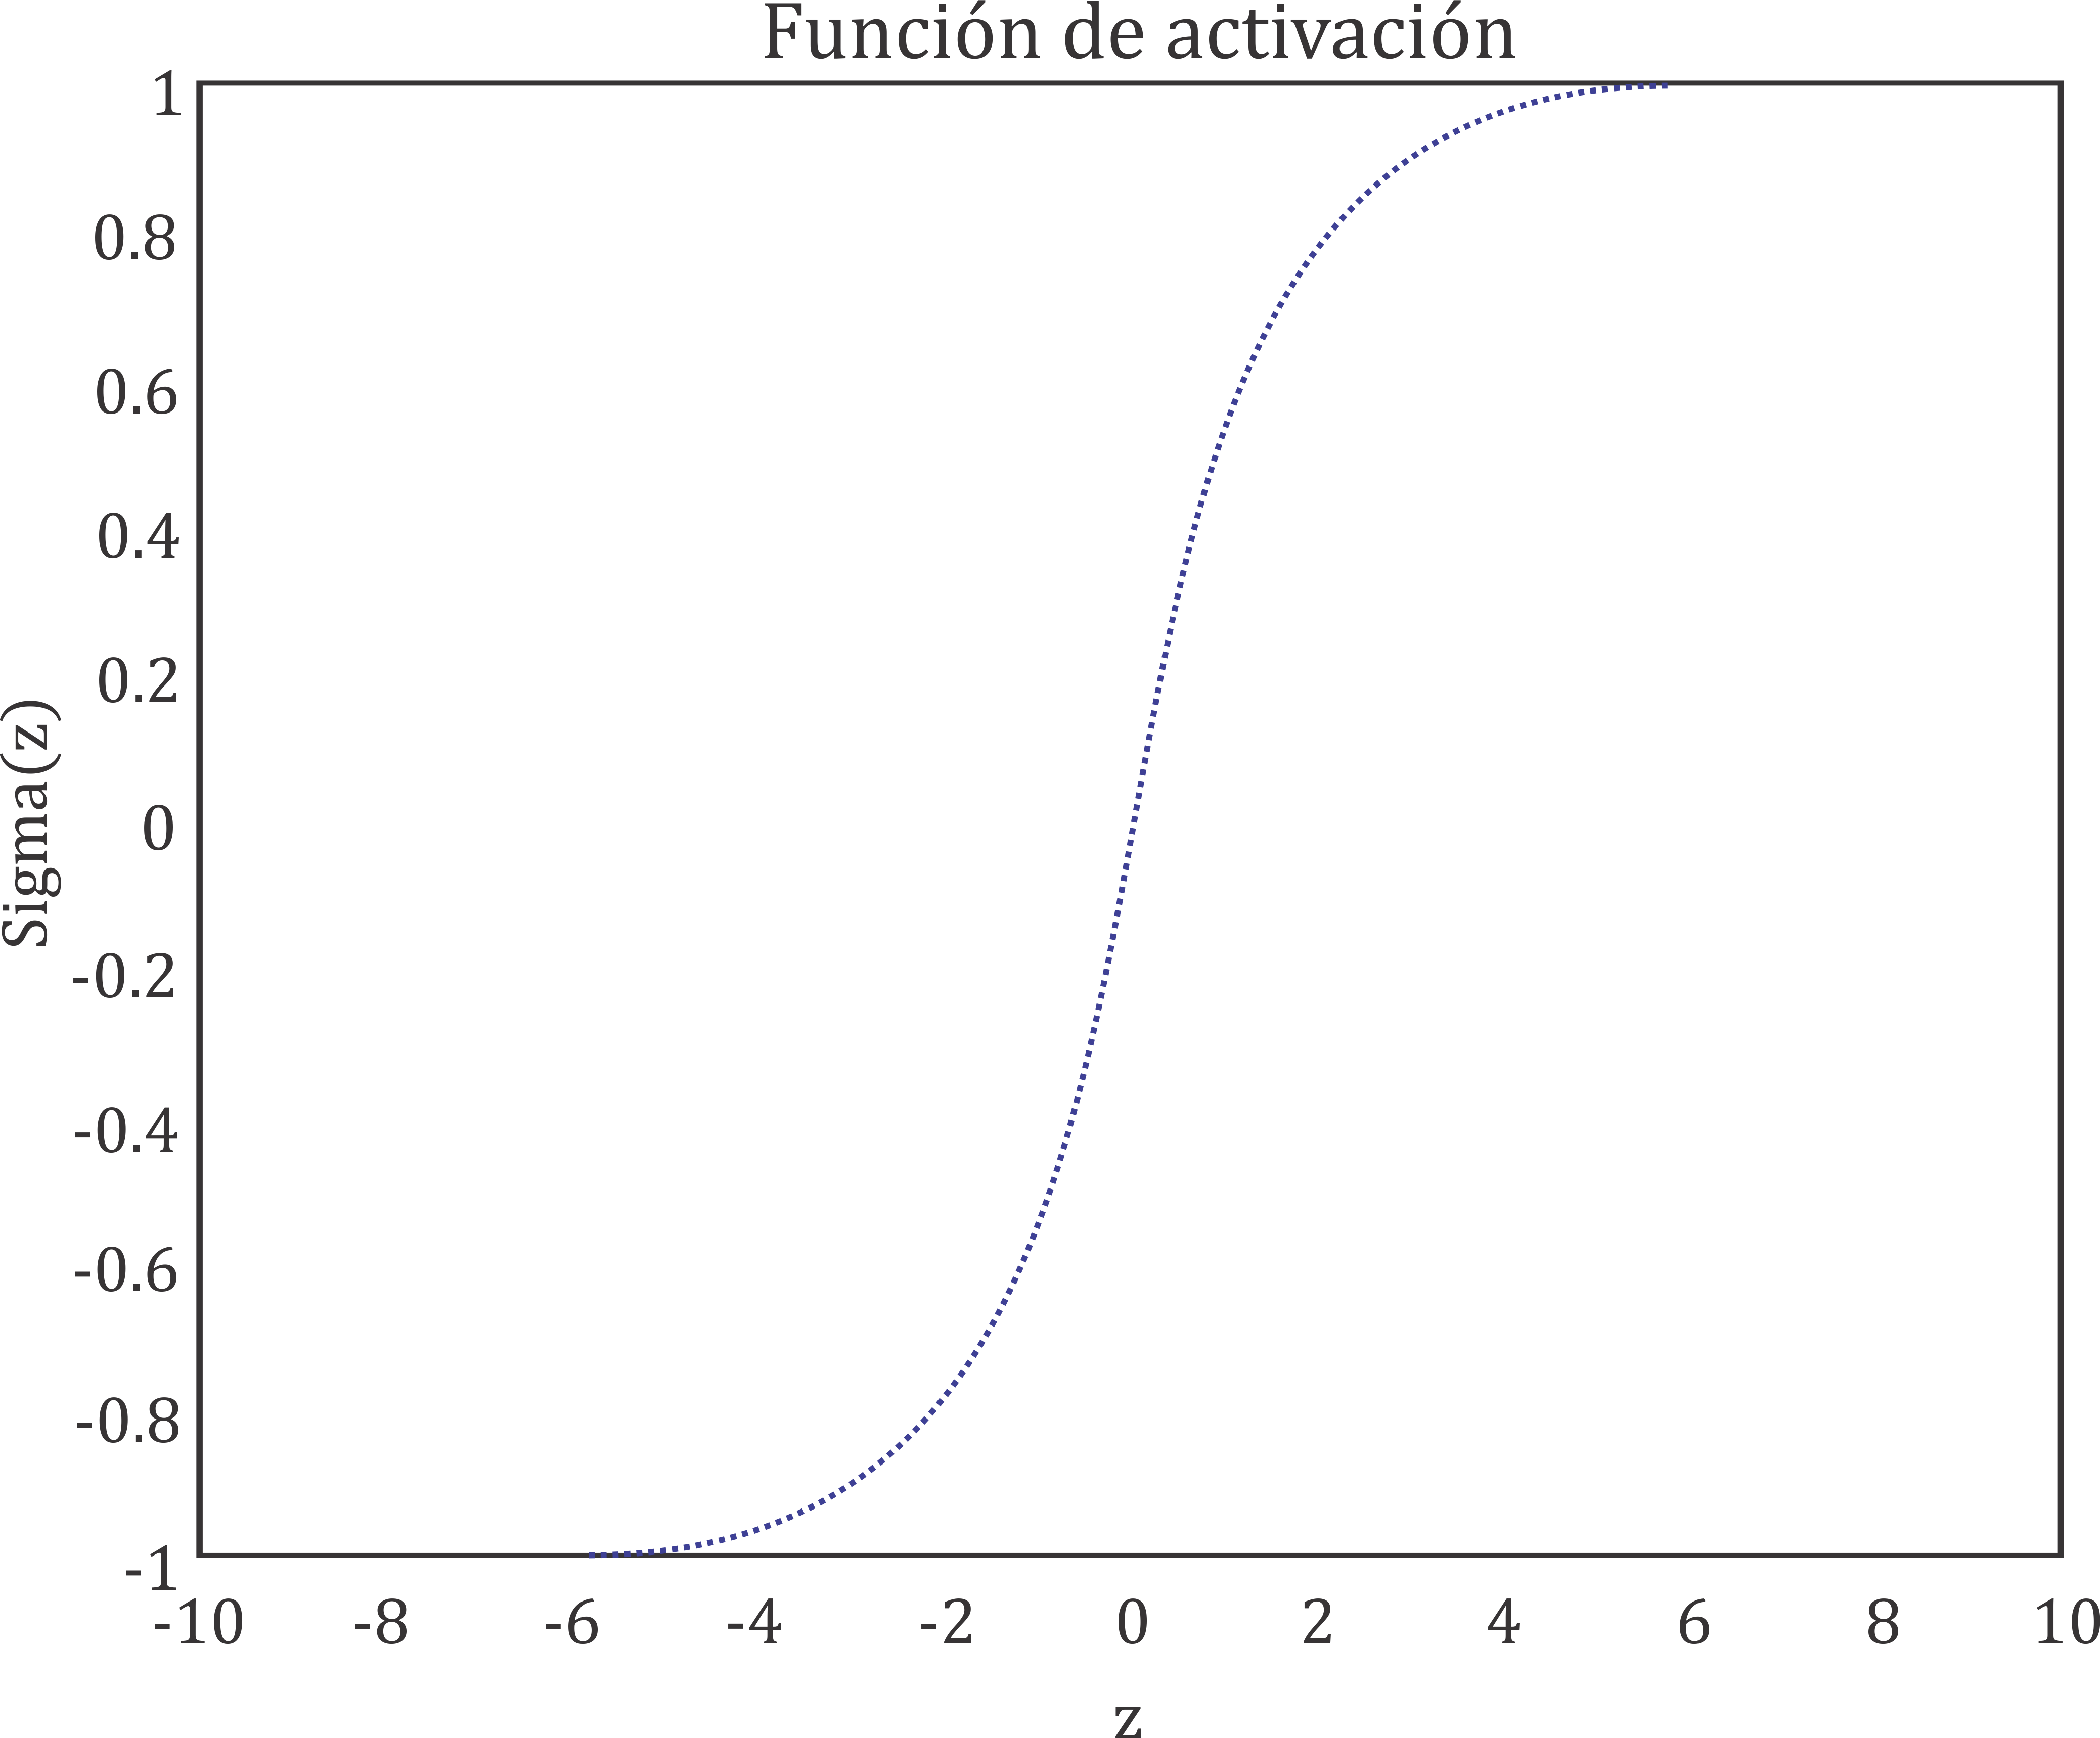
\includegraphics[width=5cm]{img/fig_activationFunction.png}
	\caption{Gr\'afica de  la funci\'on de activaci\'on.}
	\label{fig:activa}
\end{figure}

Se considera una RNA de tres capas cuya topolog\'ia se
muestra en la figura \ref{fig:percep}.  

\begin{figure}[H]
	\centering
	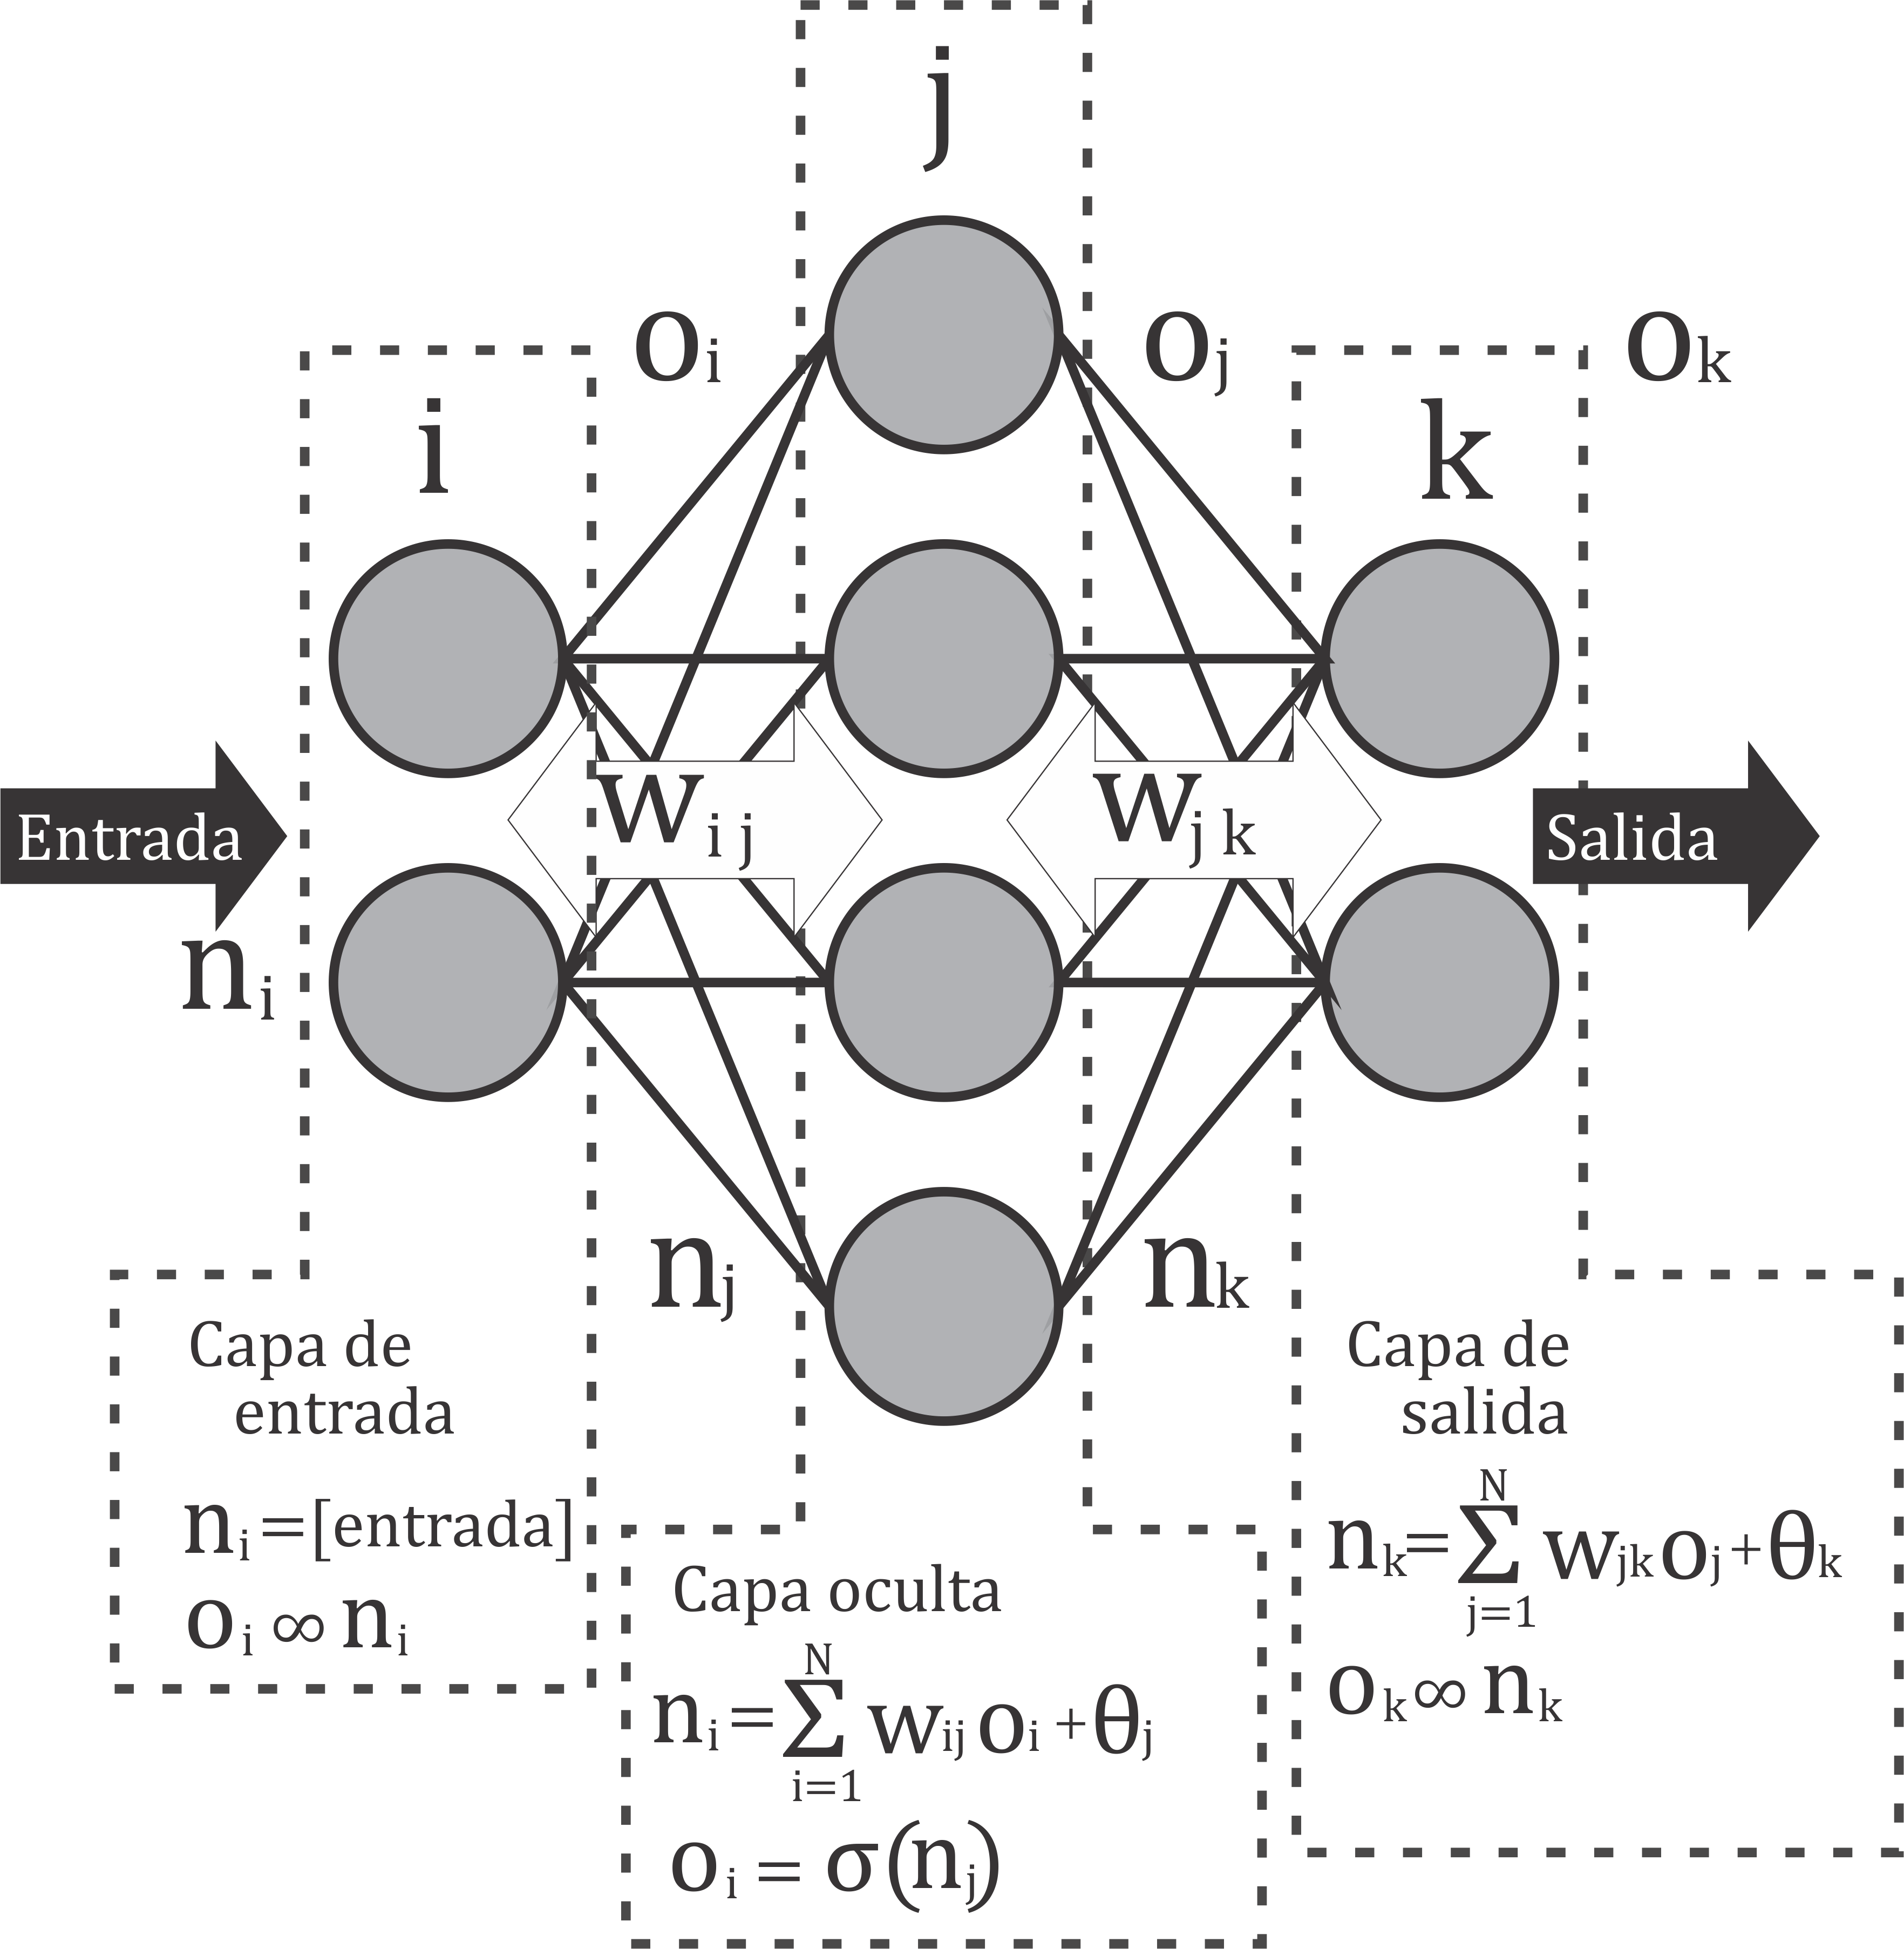
\includegraphics[width=5cm]{img/fig_perceptron.png}
	\caption{Topolog\'ia de la RNA con capa de entrada, oculta y salida.}
	\label{fig:percep}
\end{figure}

Los indices $i$, $j$ y $k$ se asocian con las neuronas de la capa
de entrada, oculta y salida, respectivamente. Adem\'as, $n_i$ representa
la entrada de la $i$-\'esima neurona, y $o_i$ su correspondiente
salida. La entrada-salida propiedad de cada neurona
matem\'aticamente se expresa como: 

\begin{equation}
	o_i=\sigma(n_i)
	\label{entrada}
\end{equation}
\begin{equation}
	o_j=\sigma(n_j)
	\label{oculta}
\end{equation}
\begin{equation}
	o_k=\sigma(n_k)
	\label{salida}
\end{equation}

Las entradas a cada distinto tipo de neurona dependiendo
de la capa a la que pertenece, se expresa de siguiente forma:

\begin{equation}
	n_i=\text{est\'imulos ambientales de la RNA} \label{estimulo}
\end{equation}
\begin{equation}
	n_j=\sum^{N_i}_{i=1}w_{ij}o_i+\theta_j
\end{equation}
\begin{equation}
	n_k=\sum^{N_j}_{j=1}w_{jk}o_j+\theta_k
\end{equation}

$N_i$ y $N_j$ representan el n\'umero de unidades que forman
las capas de entrada y oculta respectivamente, mientras que
$w_{ij}$ es el peso sin\'aptico que determina la fuerza de conexi\'on
entre las neuronas $i$ y $j$. Por \'ultimo, el par\'ametro de umbral
relacionado con la neurona $j$ se representa por $\theta_j$.

La RNA representar\'a la funci\'on de onda, la funci\'on sigmoidal
solo se emplea en la capa oculta con el fin de suavizar
y moderar la respuesta de la red. La respuesta total por parte
de la red esta dada por:

\begin{equation}
	o_k=\sum^{N_j}_{j=1}w_{jk}\sigma(\sum^{N_i}_{i=1}w_{ij}n_i+\theta_j)+\theta_k
\end{equation}

Al derivar $o_k$ con respecto a los par\'ametros que definen
el comportamiento de la red se obtiene el siguiente conjunto
de ecuaciones:

\begin{equation}
	\frac{\partial o_k}{\partial w_{ij}}=w_{jk}\sigma' (n_j)n_i
\end{equation}
\begin{equation}
	\frac{\partial o_k}{\partial w_{jk}}=\sigma (n_j)\delta_{kk'}
\end{equation}
\begin{equation}
	\frac{\partial o_k}{\partial \theta_j}=w_{jk}\sigma' (n_j)
\end{equation}
\begin{equation}
	\frac{\partial o_k}{\partial \theta_k}=\delta_{kk'}
\end{equation}


Cada una de estas ecuaciones juega un papel importante
en el proceso de aprendizaje de la RNA. Esta informaci\'on
de razones de cambio indican las direcciones correctas para
ajustar los par\'ametros que permiten sintonizar la respuesta de
la red lo mas pr\'oxima posible a una respuesta deseada. Resta
considerar las derivadas de la salida de la red con respecto a
las entradas o est\'imulos recibidos por la red, en general estas
se expresan:

\begin{equation}
	\frac{\partial^\lambda o_k}{\partial n_i^\lambda}=\sum^{N_j}_{j=1}w_{jk}\sigma^\lambda(n_j)w_{ij}^\lambda
	\label{lamda}
\end{equation}
